\documentclass[10pt]{article}

\usepackage{fontspec}
\usepackage{unicode-math}
\usepackage{xcolor}
\usepackage{tikz}
\usetikzlibrary{positioning,calc,arrows.meta,patterns}

\setsansfont{KoPubWorld Dotum_Pro}[
  Path=fonts/,
  Extension=.otf,
  UprightFont={* Light},
  BoldFont={* Bold}
]
\setmainfont{KoPubWorld Batang_Pro}[
  Path=fonts/,
  Extension=.otf,
  UprightFont={* Light},
  BoldFont={* Bold}
]
\setmathfont{Latin Modern Math}

\usepackage[
  paperwidth=182mm,paperheight=257mm,
  top=22mm,bottom=25mm,inner=22mm,outer=18mm
]{geometry}

% 공통 흑백 TikZ 도해 스타일.
% 최종 인쇄 도판의 가장 작은 글자는 6.5pt 이상으로 고정한다.
\newcommand{\DiagramMinFontSize}{6.5}
\newcommand{\DiagramBodyFont}{\sffamily\fontsize{6.5pt}{7.4pt}\selectfont}
\newcommand{\DiagramTitleFont}{\sffamily\bfseries\fontsize{8pt}{9.2pt}\selectfont}

\tikzset{
  diagram/.style={x=1cm,y=1cm,>=Stealth},
  diagram panel/.style={draw=black!65,fill=black!1,line width=0.55pt,rounded corners=1.6mm},
  diagram panel title/.style={font=\DiagramTitleFont,anchor=west,text=black},
  depth label/.style={font=\DiagramBodyFont,anchor=south,text=black!72},
  depth guide/.style={draw=black!24,line width=0.35pt,densely dashed},
  gate/.style={
    draw=black!72,fill=white,line width=0.55pt,rounded corners=0.9mm,
    minimum height=5.2mm,inner xsep=0.8mm,inner ysep=0.5mm,
    align=center,font=\DiagramBodyFont
  },
  path gate/.style={gate,fill=black!15,draw=black,line width=0.9pt},
  gate group/.style={draw=black!45,line width=0.45pt,densely dashed,rounded corners=1.1mm},
  wire/.style={draw=black!62,line width=0.55pt,-{Stealth[length=1.7mm,width=1.2mm]}},
  path wire/.style={draw=black,line width=1.05pt,-{Stealth[length=1.9mm,width=1.35mm]}},
  diagram note/.style={font=\DiagramBodyFont,text=black!78,align=left},
  diagram footer/.style={font=\DiagramBodyFont,text=black,align=center}
}


\newenvironment{bookfigure}[2]
  {\begin{center}\sffamily\bfseries #1\par\medskip\normalfont}
  {\end{center}}

\pagestyle{empty}

\begin{document}
\begin{bookfigure}{같은 \(c_4\)를 만드는 사슬과 펼친 식}{fig:ch04-chain-vs-expanded}
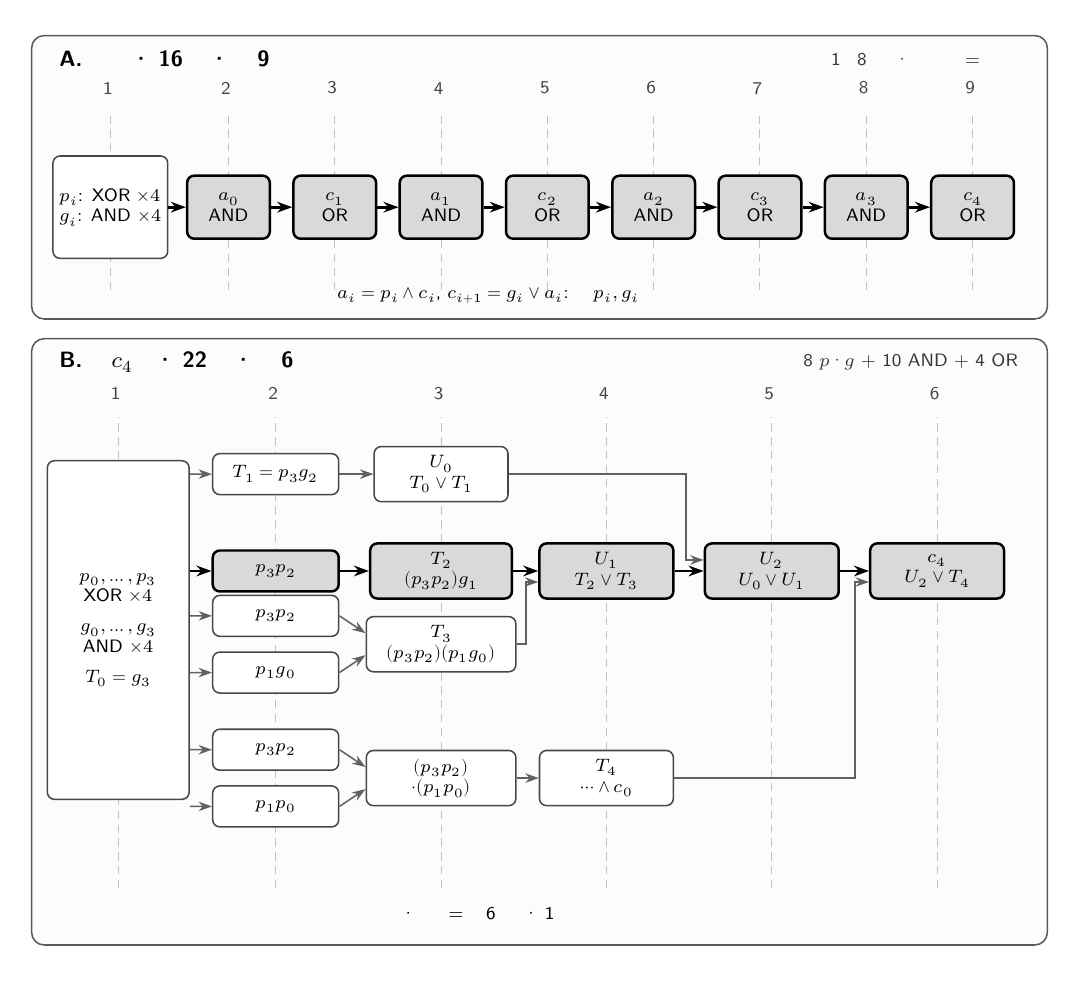
\begin{tikzpicture}[diagram]
  \path[use as bounding box] (0,0) rectangle (13.0,11.75);

  % ------------------------------------------------------------------
  % A. Ripple carry: 8 p/g gates + 8 carry gates = 16, depth 9.
  % The p/g gates are grouped because they are all evaluated in layer 1.
  % ------------------------------------------------------------------
  \draw[diagram panel] (0.05,8.05) rectangle (12.95,11.65);
  \node[diagram panel title] at (0.28,11.35)
    {A. 리플 캐리 · 16게이트 · 최장 9층};
  \node[diagram note,anchor=east] at (12.70,11.35)
    {1층은 8개 묶음 · 이후 상자 하나 = 게이트 하나};

  \foreach \x/\label in {
    1.05/1층,2.55/2층,3.90/3층,5.25/4층,6.60/5층,
    7.95/6층,9.30/7층,10.65/8층,12.00/9층}
  {
    \node[depth label] at (\x,10.78) {\label};
    \draw[depth guide] (\x,8.42) -- (\x,10.68);
  }

  % gate:ripple-pg
  % gate:ripple-pg
  % gate:ripple-pg
  % gate:ripple-pg
  % gate:ripple-pg
  % gate:ripple-pg
  % gate:ripple-pg
  % gate:ripple-pg
  \node[gate,minimum width=14mm,minimum height=13mm] (r-pg) at (1.05,9.47)
    {\(p_i\): XOR \(\times4\)\\
     \(g_i\): AND \(\times4\)};

  % gate:ripple-carry
  \node[path gate,minimum width=10.5mm,minimum height=8mm] (r-a0) at (2.55,9.47)
    {\(a_0\)\\AND};
  % gate:ripple-carry
  \node[path gate,minimum width=10.5mm,minimum height=8mm] (r-c1) at (3.90,9.47)
    {\(c_1\)\\OR};
  % gate:ripple-carry
  \node[path gate,minimum width=10.5mm,minimum height=8mm] (r-a1) at (5.25,9.47)
    {\(a_1\)\\AND};
  % gate:ripple-carry
  \node[path gate,minimum width=10.5mm,minimum height=8mm] (r-c2) at (6.60,9.47)
    {\(c_2\)\\OR};
  % gate:ripple-carry
  \node[path gate,minimum width=10.5mm,minimum height=8mm] (r-a2) at (7.95,9.47)
    {\(a_2\)\\AND};
  % gate:ripple-carry
  \node[path gate,minimum width=10.5mm,minimum height=8mm] (r-c3) at (9.30,9.47)
    {\(c_3\)\\OR};
  % gate:ripple-carry
  \node[path gate,minimum width=10.5mm,minimum height=8mm] (r-a3) at (10.65,9.47)
    {\(a_3\)\\AND};
  % gate:ripple-carry
  \node[path gate,minimum width=10.5mm,minimum height=8mm] (r-c4) at (12.00,9.47)
    {\(c_4\)\\OR};

  \draw[path wire] (r-pg.east) -- (r-a0.west);
  \draw[path wire] (r-a0.east) -- (r-c1.west);
  \draw[path wire] (r-c1.east) -- (r-a1.west);
  \draw[path wire] (r-a1.east) -- (r-c2.west);
  \draw[path wire] (r-c2.east) -- (r-a2.west);
  \draw[path wire] (r-a2.east) -- (r-c3.west);
  \draw[path wire] (r-c3.east) -- (r-a3.west);
  \draw[path wire] (r-a3.east) -- (r-c4.west);

  \node[diagram footer] at (6.50,8.35)
    {\(a_i=p_i\land c_i\), \(c_{i+1}=g_i\lor a_i\): 직접 \(p_i,g_i\) 선은 생략하고 올림 경로만 그렸다};

  % ------------------------------------------------------------------
  % B. Expanded c4: 8 p/g + 10 AND + 4 OR = 22, depth 6.
  % Direct inputs such as g1 and c0 are written inside their destination
  % gates. Only dependencies between intermediate gates are drawn.
  % ------------------------------------------------------------------
  \draw[diagram panel] (0.05,0.10) rectangle (12.95,7.80);
  \node[diagram panel title] at (0.28,7.50)
    {B. 펼친 \(c_4\) 식 · 22게이트 · 최장 6층};
  \node[diagram note,anchor=east] at (12.70,7.50)
    {8 \(p\)·\(g\) + 10 AND + 4 OR};

  \foreach \x/\label in {1.15/1층,3.15/2층,5.25/3층,7.35/4층,9.45/5층,11.55/6층}
  {
    \node[depth label] at (\x,6.90) {\label};
    \draw[depth guide] (\x,0.82) -- (\x,6.80);
  }

  % gate:expanded-pg
  % gate:expanded-pg
  % gate:expanded-pg
  % gate:expanded-pg
  % gate:expanded-pg
  % gate:expanded-pg
  % gate:expanded-pg
  % gate:expanded-pg
  \node[gate,minimum width=18mm,minimum height=43mm] (e-pg) at (1.15,4.10)
    {\(p_0,\ldots,p_3\)\\XOR \(\times4\)\\[1.2mm]
     \(g_0,\ldots,g_3\)\\AND \(\times4\)\\[1.2mm]
     \(T_0=g_3\)};

  % Six layer-2 AND gates.
  % gate:expanded-and
  \node[gate,minimum width=16mm] (e-t1) at (3.15,6.08) {\(T_1=p_3g_2\)};
  % gate:expanded-and
  \node[path gate,minimum width=16mm] (e-t2a) at (3.15,4.85) {\(p_3p_2\)};
  % gate:expanded-and
  \node[gate,minimum width=16mm] (e-t3a) at (3.15,4.28) {\(p_3p_2\)};
  % gate:expanded-and
  \node[gate,minimum width=16mm] (e-t3b) at (3.15,3.56) {\(p_1g_0\)};
  % gate:expanded-and
  \node[gate,minimum width=16mm] (e-t4a) at (3.15,2.58) {\(p_3p_2\)};
  % gate:expanded-and
  \node[gate,minimum width=16mm] (e-t4b) at (3.15,1.86) {\(p_1p_0\)};

  % Layer 3: one OR and three AND gates.
  % gate:expanded-or
  \node[gate,minimum width=17mm,minimum height=7mm] (e-u0) at (5.25,6.08)
    {\(U_0\)\\\(T_0\lor T_1\)};
  % gate:expanded-and
  \node[path gate,minimum width=18mm,minimum height=7mm] (e-t2) at (5.25,4.85)
    {\(T_2\)\\\((p_3p_2)g_1\)};
  % gate:expanded-and
  \node[gate,minimum width=19mm,minimum height=7mm] (e-t3) at (5.25,3.92)
    {\(T_3\)\\\((p_3p_2)(p_1g_0)\)};
  % gate:expanded-and
  \node[gate,minimum width=19mm,minimum height=7mm] (e-t4c) at (5.25,2.22)
    {\((p_3p_2)\)\\\(\cdot(p_1p_0)\)};

  % Layer 4: U1 and T4 become ready independently.
  % gate:expanded-or
  \node[path gate,minimum width=17mm,minimum height=7mm] (e-u1) at (7.35,4.85)
    {\(U_1\)\\\(T_2\lor T_3\)};
  % gate:expanded-and
  \node[gate,minimum width=17mm,minimum height=7mm] (e-t4) at (7.35,2.22)
    {\(T_4\)\\\(\cdots\land c_0\)};

  % Layer 5 and 6: finish the arrival-time-aware OR tree.
  % gate:expanded-or
  \node[path gate,minimum width=17mm,minimum height=7mm] (e-u2) at (9.45,4.85)
    {\(U_2\)\\\(U_0\lor U_1\)};
  % gate:expanded-or
  \node[path gate,minimum width=17mm,minimum height=7mm] (e-c4) at (11.55,4.85)
    {\(c_4\)\\\(U_2\lor T_4\)};

  % Inputs from layer 1 to the six layer-2 gates. These are short,
  % separated horizontal segments, so no wire crosses a gate or label.
  \draw[wire] ([yshift=19.8mm]e-pg.east) -- (e-t1.west);
  \draw[path wire] ([yshift=7.5mm]e-pg.east) -- (e-t2a.west);
  \draw[wire] ([yshift=1.8mm]e-pg.east) -- (e-t3a.west);
  \draw[wire] ([yshift=-5.4mm]e-pg.east) -- (e-t3b.west);
  \draw[wire] ([yshift=-15.2mm]e-pg.east) -- (e-t4a.west);
  \draw[wire] ([yshift=-22.4mm]e-pg.east) -- (e-t4b.west);

  % T0 arrives directly from layer 1 and is written inside U0. Drawing its
  % long bypass wire would obscure the layer-to-layer flow.
  \draw[wire] (e-t1.east) -- (e-u0.west);
  \draw[path wire] (e-t2a.east) -- (e-t2.west);
  \draw[wire] (e-t3a.east) -- ([yshift=1.4mm]e-t3.west);
  \draw[wire] (e-t3b.east) -- ([yshift=-1.4mm]e-t3.west);
  \draw[wire] (e-t4a.east) -- ([yshift=1.4mm]e-t4c.west);
  \draw[wire] (e-t4b.east) -- ([yshift=-1.4mm]e-t4c.west);

  \draw[path wire] (e-t2.east) -- (e-u1.west);
  \draw[wire] (e-t3.east) -- ++(0.12,0) |- ([yshift=-1.4mm]e-u1.west);
  \draw[wire] (e-t4c.east) -- (e-t4.west);
  \draw[wire] (e-u0.east) -- ++(2.25,0) |- ([yshift=1.4mm]e-u2.west);
  \draw[path wire] (e-u1.east) -- (e-u2.west);
  \draw[path wire] (e-u2.east) -- (e-c4.west);
  \draw[wire] (e-t4.east) -- ++(2.30,0) |- ([yshift=-1.4mm]e-c4.west);

  \node[diagram footer] at (6.50,0.50)
    {굵은 선·회색 상자 = 최장 6층 경로 · 1층에서 직접 오는 입력은 도착 게이트 안에 적었다};
\end{tikzpicture}
\end{bookfigure}

\end{document}
